\documentclass[10pt,letterpaper]{article}
\usepackage[utf8]{inputenc}
\usepackage[T1]{fontenc}
\usepackage{geometry}
\geometry{margin=0.75in}
\usepackage{paracol}
\usepackage{enumitem}
\setlist[itemize]{leftmargin=*,noitemsep,topsep=0pt}
\usepackage{sectsty}
\sectionfont{\centering\bfseries\large}
\subsectionfont{\bfseries\small}
\usepackage{graphicx}
\usepackage{caption}
\usepackage{xcolor}
\definecolor{titleblue}{RGB}{0,51,102}
\usepackage{titlesec}
\titleformat{\section}{\centering\large\bfseries\color{titleblue}}{}{0em}{}
\titleformat{\subsection}{\small\bfseries\color{titleblue}}{}{0em}{}
\usepackage{noto}
\usepackage{parskip}
\setlength{\parindent}{0pt}

\begin{document}

\begin{center}
{\Huge \textbf{Timeslip: An Interactive Paracosm}} \\
\vspace{0.2cm}
{\large A Science Fiction Saga of Control and Rebellion} \\
\vspace{0.3cm}
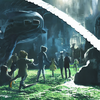
\includegraphics[width=0.8\textwidth]{title_image.jpg} % Placeholder for Stable Diffusion title image
\captionof{figure}{Concept art for the Tower World, generated by Stable Diffusion.}
\end{center}

\begin{paracol}{2}
\section{Premise}
In a far-future bureaucracy where roles stifle exploration, Ethnographer Maxim Kammerer is sent to a medieval planet ruled by Thought Control Towers that induce daily ecstatic fits. Immune to disease via nanobots, he navigates a grimy world of political intrigue and hidden tech, questioning his non-interference mandate. The saga continues in \textit{The Call from Ankyra}, where Maxim faces Arkanar's mud-soaked conspiracies, echoing his past failures.

\subsection{Themes}
\begin{itemize}
    \item Myopic Roles: Specialization blinds individuals.
    \item Institutional Stoicism: Emotion suppressed for duty.
    \item Commodified Transcendence: Ecstasy as control.
    \item Ethics of Interference: Freedom vs. stability.
\end{itemize}

\section{Worldbuilding}
\subsection{Tower World}
\begin{itemize}
    \item \textbf{Tech}: Screenless; radio-like systems; no roads.
    \item \textbf{Towers}: Broadcast mind-control signals.
    \item \textbf{Aesthetic}: Mud, slime, bodily fluids; inspired by 2007 \textit{Hard to Be a God} film.
\end{itemize}
\subsection{Ankyra}
\begin{itemize}
    \item \textbf{Setting}: Medieval Arkanar; Gray Cloaks hunt intellectuals.
    \item \textbf{Tech}: Hidden beacon arrays; Wanderer relics.
    \item \textbf{Aesthetic}: Rain, decay, visceral chaos.
\end{itemize}
\subsection{Outerworld}
\begin{itemize}
    \item Sterile COMCON-2 bureaucracy; encrypted comms.
    \item Visual contrast: Clean whites vs. planetary grime.
\end{itemize}

\switchcolumn

\section{Characters}
\begin{itemize}
    \item \textbf{Maxim Kammerer}: Ethnographer; haunted by past interventions.
    \item \textbf{Calyra}: Prodigy loyalist; neurologically conditioned.
    \item \textbf{Quiet Mechanic}: Dissident; knows tower origins.
    \item \textbf{Ryn}: Apprentice; partially immune.
    \item \textbf{Ari}: Tower network AI; fragmented.
    \item \textbf{Shavri}: Weaver; escapes to Outerworld.
    \item \textbf{Rumata}: Progressor noble in Ankyra.
    \item \textbf{Outerworld}: Dr. Keryn Thal, Rolen Mirsk, Myra Kade, Archive Node 7.
\end{itemize}

\begin{center}
\includegraphics[width=0.45\textwidth]{character_image.jpg} % Placeholder for Stable Diffusion character art
\captionof{figure}{Maxim Kammerer in Tower World, generated by Stable Diffusion.}
\end{center}

\section{Episode Guide}
\subsection{Sanity Check}
\textbf{Season 1: Landing in the Blind}
\begin{enumerate}
    \item \textit{Briefing Room}: Orbital drop; first Call.
    \item \textit{Masks for the Living}: Market; Shavri appears.
    \item \textit{The First Pulse}: Subharmonic recorded.
    \item \textit{The Mechanic’s Puzzle}: Meets Mechanic.
    \item \textit{Paper in the Rain}: Shavri’s coded weaves.
    \item \textit{Test of Faith}: Shrine performance.
    \item \textit{The Malfunction}: Tower silence.
    \item \textit{Flight Path}: Shavri’s sky-track.
    \item \textit{Extraction Point}: Shavri escapes.
\end{enumerate}

\textbf{Season 2: The Shadow Signal}
\begin{enumerate}
    \item \textit{River of Ash}: Hinterland rituals.
    \item \textit{Calyra}: Orator emerges.
    \item \textit{Cracks in the Crystal}: Ryn’s repairs.
    \item \textit{Ledger Error}: Obeyed chaos.
    \item \textit{The Scholar’s Garden}: Forbidden truths.
    \item \textit{Through the Furnace}: Signal whisper.
    \item \textit{Festival of Dawn}: Synchronized Call.
    \item \textit{The Mechanic’s Oath}: Fix or break.
    \item \textit{The Voice in the Static}: “I see you.”
\end{enumerate}

\switchcolumn

\textbf{Season 3: The Resonance}
\begin{enumerate}
    \item \textit{The Call}: City convulsion.
    \item \textit{The Quiet Mechanic}: Pre-tower tech.
    \item \textit{Calyra’s Rise}: Pulse-synced rhetoric.
    \item \textit{Apprentice}: Ryn’s immunity.
    \item \textit{The Scholar}: Ritual breakdown.
    \item \textit{The Hidden Voice}: Ari warns.
    \item \textit{Imported Chains}: Offworld tech.
    \item \textit{The Unbinding}: Plan risks Ari.
    \item \textit{The Last Broadcast}: Towers disabled.
\end{enumerate}

\textbf{Season 4: The Last Frequency}
\begin{enumerate}
    \item \textit{Static Bloom}: Ari recontacts.
    \item \textit{Counter-Harmonics}: Sub-signals.
    \item \textit{The Scholar’s Secret}: Beacons repurposed.
    \item \textit{Ecstasy’s Edge}: Catatonia case.
    \item \textit{The Voice Revealed}: AI revealed.
    \item \textit{Break or Mend}: Sabotage vs. repair.
    \item \textit{Calyra’s Choice}: Council test.
    \item \textit{The Ninth Tower}: Alien core.
    \item \textit{Orders from COMCON-2}: Ankyra mission.
\end{enumerate}

\subsection{The Call from Ankyra}
\textbf{Season 1: The Mud of Arkanar}
\begin{enumerate}
    \item \textit{Arrival in Disguise}: Anton in grime.
    \item \textit{The Gray Cloaks}: Intellectual hunt.
    \item \textit{The Feast and the Gutter}: Noble rot.
    \item \textit{Letters from Calyra}: Tower parallels.
    \item \textit{Gods and Mud}: Rumata’s disdain.
    \item \textit{The Scholar’s Trial}: Sham justice.
    \item \textit{Masks of Power}: Beacon array.
    \item \textit{A God’s Temptation}: Save scholars.
    \item \textit{Blood in the Rain}: Coup chaos.
\end{enumerate}

\textbf{Season 2: The Price of Interference}
\begin{enumerate}
    \item \textit{After the Coup}: Splintered Cloaks.
    \item \textit{The Black Archive}: Crystal core.
    \item \textit{The Disease of Memory}: Plague echoes.
    \item \textit{Rumata’s Oath}: Progressor reveal.
    \item \textit{Calyra’s Last Letter}: Tower collapse.
    \item \textit{The Festival of Knives}: Extraction.
    \item \textit{Ari’s Echo}: Fragmented voice.
    \item \textit{The Final Intervention}: Beacon down.
    \item \textit{The Mud Beyond}: Recall; Ari’s signal.
\end{enumerate}

\switchcolumn

\section{Production Notes}
\begin{itemize}
    \item \textbf{Visuals}: Grime, slime, rust; clean Outerworld contrast. Use Noto fonts for alien inscriptions.
    \item \textbf{Sound}: Dripping, coughing, bells; static for comms.
    \item \textbf{Shooting}: Close-ups on filth; nanobot immunity shown via Maxim’s calm handling.
    \item \textbf{Echoes}: Tower guards → Gray Cloaks; Ari → relic signals.
    \item \textbf{Reappearances}: Shavri (S1–S2, Ankyra S2); Calyra (S2–S4, letters); Ari (S3–S4, Ankyra S2).
\end{itemize}

\begin{center}
\includegraphics[width=0.45\textwidth]{world_image.jpg} % Placeholder for Stable Diffusion world art
\captionof{figure}{Arkanar’s muddy streets, generated by Stable Diffusion.}
\end{center}

\end{paracol}

\end{document}
